\documentclass{standalone}
\usepackage{standalone}

\begin{document}
\chapter{Introduction}
\label{chap:intro}
\section{Background}
 From the current research trends, it has become clear that extracting linguistic information from natural language or text is an powerful method to create a robust and accurate natural language processing system. Parts of Speech(POS) is one of the basic linguistic information that we can extract from texts as a useful feature. Once POS Tagging was done by hand but now is done in the context of computer linguistics. POS Tagging is the process of tagging the words in a document or text according to their corresponding Parts Of Speech based on their context and definition. It is not an easy or straightforward task as the tag of a word varies based on their language, sentence, etc. In the Bengali language, it is harder to define the POS Tag of a sentence as Bengali follows more complex rules. Researchers Have been working on POS Tagging for a long time and in many languages, they have been able to bring a good and accurate POS Tagger. POS Taggers with high accuracy have been developed  English, German, French or other European languages\cite{cite1}\cite{cite2}\cite{cite3}\cite{cite4}. But in Bengali, there had not been any such significant success.
Parts of speech tagging in Bengali is harder than just having sentences of words and giving them a tag. Due to complex rules in Bengali, it is hard to design good rule-based tagger for Bengali. POS tagging techniques are mainly of two types, rule-based and stochastics. Various statistical models such as ME, HMM, CRF, SVM  has been applied to date but neither of them shows that much good accuracy in tagging. Besides most of them depends on tools like stemmer. That means the accuracy of these methods depends on the accuracy of the stemmers. It is also hard to create a correct dataset because Bengali is such a complex language that tagging by a human can not always ensure a correct tag. Due to diverse expression in the Bengali language in different platforms, it is also possible for the same sentence to have two different tagset. This also makes this task a bit more challenging.
\section{Motivation}
In Natural Language Processing, most models are based on the bag of words or tokens. So having some features extracted or finding some pattern in the words or sentences always give the research an advantage. Parts of Speech is such kind of features that we may not need or use directly or practically but it can be used as an important feature in several NLP researches.n Natural Language Processing hierarchy\footnote{https://en.wikipedia.org/wiki/Natural_language_processing#Major_tasks_in_NLP}, at the bottom,  is a sentence and word segmentation . POS is at the top of it, so having pos tagged data can help in building parse trees  that can be used for several NLP systems.
\subsection{Word Sense Disambiguation}
A natural language text can have multiple meanings or senses according to their context. The task of WSD or Word Sense Disambiguation is to sense the correct meaning of natural language text based on their context \cite{cite5} \cite{cite6}.POS Tagging plays an important role in Word Sense Disambiguation.\\
\begin{figure}[h!]
\centering
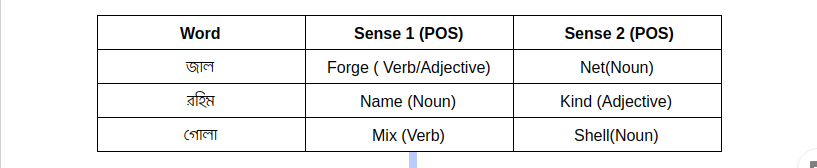
\includegraphics[width=1.0\columnwidth]{img/WSD.png}
\caption{Word Sense Disambiguation example}
\label{WSD}
\end{figure}
\\
 So from the examples in figure \ref{WSD}, we can see that same word can have different senses and they can be distinguished by knowing their Parts of Speech.
\subsection{Text to Speech Conversion}
In Bengali pronunciation  of the different words can be the same. They can only be distinguished based on their context or meaning. Parts of speech of a word can help in this case. Based on the parts of speech of a word in a text we can get the real sense of a word in the text and then it can be used to convert into speech.
\subsection{Named Entity Recognition}
Named Entity Recognition (NER) is a Information Retrieval subtask that finds and categorizes the named entity in a sentence in some predefined classes.\\
\begin{figure}[h!]
\centering
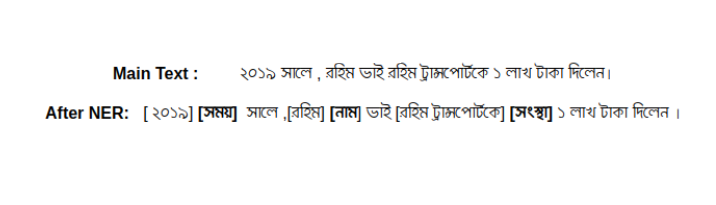
\includegraphics[width=1.0\columnwidth]{img/NER1.png}
\caption{Named Entity Recognition example}
\label{NER}
\end{figure}
\\
The figure \ref{NER} shows a Bengali NER example.\\
So in order to find the NER, we need to find the nouns in the sentence, only then we can classify them. That is why we need a good POS Tagger.
\subsection{Sentimental Analysis}
In Sentimental Analysis, we basically try to find what the sentence refers to, positive or negative sentiment. In this sector, POS is one of the most important features. POS can help to define the positive or negative sense of a text. Yes it can be possible to do this without POS tagging , but in many cases system will face problems that can be solved with tagged POS.\footnote{https://www.quora.com/What-is-the-use-and-need-of-part-of-speech-POS-tagging-in-sentimental-analysis}
\subsection{Question Answering}
Question Answering is an NLP Discipline in the field of information retrieval\footnote{https://en.wikipedia.org/wiki/Question_answering}. In Question Answering System POS tagging is used as an important feature. POS can be a piece of useful information for a QA system. It helps understand the context of questions and to generate the answer.

\section{Overview}
In this report, we have discussed some of the previous works conducted on this topic in the Literature Review. We have tried to specify the problems that are still on the system.Then we have discussed our proposed method. In the Methodology chapter, we have disclosed our work methods. In the Dataset Chapter, We have given a brief note on our dataset.

\end{document}